% Construction : parallélogramme A(0,0), B(4,0), C(5.2,2.2), D(1.2,2.2).
%   La diagonale [AC] le coupe en deux triangles superposables ABC et ACD.
%   Hauteur commune h = 2.2, base commune b = 4.
% SVG : x = 20 + 44x, y = 120 - 44y.
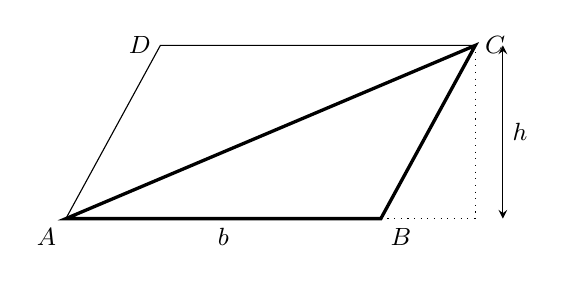
\begin{tikzpicture}[scale=1, >=stealth, every node/.style={font=\small}]
  \draw (0,0) -- (4,0) -- (5.2,2.2) -- (1.2,2.2) -- cycle;
  \draw[very thick] (0,0) -- (4,0) -- (5.2,2.2) -- cycle;
  \draw[dotted] (5.2,2.2) -- (5.2,0) node[below] {};
  \draw[<->] (5.55,0) -- (5.55,2.2) node[midway, right] {$h$};
  \draw[dotted] (4,0) -- (5.2,0);
  \node[below] at (2,0) {$b$};
  \node[below left] at (0,0) {$A$}; \node[below right] at (4,0) {$B$};
  \node[right] at (5.2,2.2) {$C$}; \node[left] at (1.2,2.2) {$D$};
\end{tikzpicture}
